% In the batch queue,  queue time becomes dominant but, at the same time, we
% have more freedom to decide the parameters of the slot.

\subsection{Experiments}

In this section we present experiments that aim to determine the performances of the NGE and to show how it provides a minimal overhead while introducing new functionalities.

Experiments consist in running AthenaMP instances by using NGE pilots where each AthenaMP simulates a pre-determined number of events taken from ATLAS workload.	
We present three groups of experiments in which we test the NGE for weak scalability, weak scalability with multiple generation and strong scalability.

We collected data about the execution time of the pilots and the AthenaMP that have been executed within them by considering all stages of the execution.
Experiments have been performed out of production by using NGE's pilots on TITAN's batch queue. 
Because of TITAN's batch queue, the turnaround time of each run of our experiments is dominated by the time spent on TITAN's queue. Since we are interested only in the performances of the NGE, we removed queue time from our statistics.

All the experiments have been performed by setting AthenaMP in such a way that it uses all the 16 cores present on TITAN's nodes. 


\subsubsection{Weak scalability}

The experiment consists in running as many AthenaMP instances (also referred as tasks from now-on) as the number of nodes controlled by the pilot. Each AthenaMP have been assigned with 100 events whose simulation requires  ~$70$ minutes. 
 
Tasks do not experience queue within the pilot since there is one node for each AthenaMP instance. Therefore, delays are consequence of only three factors: i) the bootstrapping of the pilot on the nodes; ii) the manager, as defined in Section \ref{sec:arch}, that has to dispatch tasks to the pilot; iii) the time that the agent requires to spawn all the tasks on the nodes.

We tested different pilot sizes, i.e. : 250, 500, 1000 and 2000. For all of them the walltime was 2 hours.

Figure \ref{fig:weakScal1a} depicts the average pilot duration, the average execution time of AthenaMP and pilot's overhead as function of the pilot size.  

\begin{figure}[!htb]
        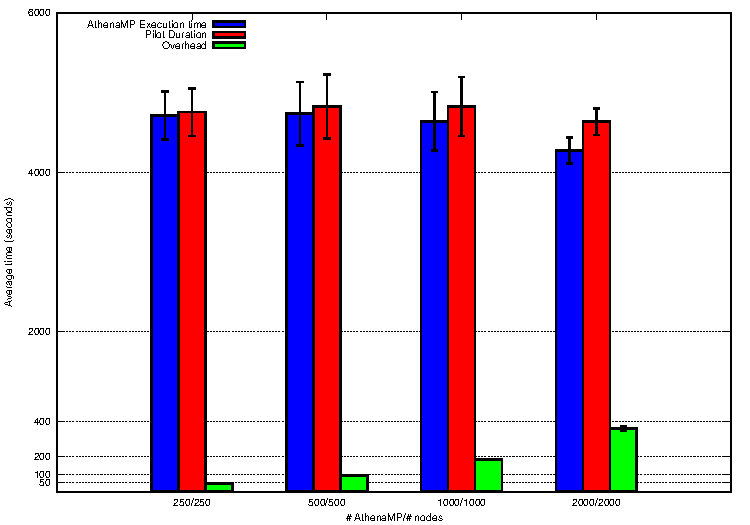
\includegraphics[height=4.5cm,width=\columnwidth]{./figures/NGE/weak1.pdf}
    \caption{Weak scalability: average pilot duration, average duration of a single AthenaMP execution and pilot's overhead for different pilot sizes (250, 500, 1000 and 2000 nodes). Note that the overhead refers to the axis on the right and it is expressed in tenths of a second.}
\label{fig:weakScal1a}
\end{figure}

Firstly, we can observe that, despite some fluctuations due to external factors\footnote{such as the Titan's shared filesystem and the shared database used by the NGE}, the average execution time of AthenaMP oscillates between 4200 and 4800 seconds. Secondly, we can observe that in all the cases the gap between AthenaMP execution times and the pilot durations is minimal although it slightly increases with the pilot size.
By observing NGE's overhead, we can notice the overhead does not grow linearly with the number of units.

%\begin{figure}[!htb]
%        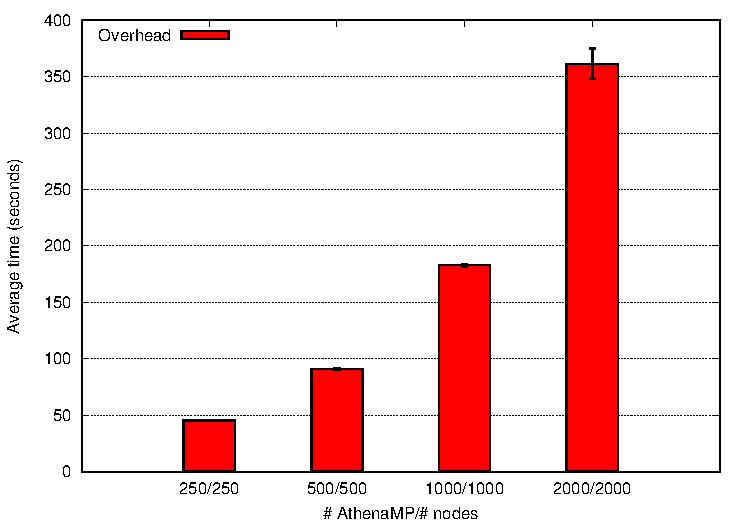
\includegraphics[width=0.4\textwidth]{./figures/NGE/weakOver1.pdf}
%    \caption{Weak scalability: average overhead by running AthenaMP on 200, 500, 1000 and 2000 nodes.}
%\label{fig:weakScal1b}
%\end{figure}


\subsubsection{Weak scalability with multiple generation }
This experiment is similar to the one presented above but in this case we want to test also the impact of submitting new AthenaMP instances in place of those that end. The reason behind this experiment is to stress pilot's components by pushing new tasks while others are ending their execution.

In order to perform the experiments in less than two hours per run, we decided to send for execution a number of AthenaMP instances equal to five times the number of nodes and we reduced  the number of events that are simulated by each Athena-MP to sixteen\footnote{Note that the number of events has been chosen in such a way that all the cores of a node run one event.}. This allows us to complete a single AthenaMP in ~20 minutes only. 

We tested different pilot sizes, i.e. : 256, 512, 1024 and 2048. For all of them the walltime was 3 hours. 

Figure \ref{fig:weakScal2a} depicts the average pilot duration, the average execution time of five sequential instances of AthenaMP and the corresponding overhead.  
We can observe that the difference between the two durations is more marked than in the previous experiments. Despite this we can notice that the growth of the overhead is still less than linear.

\begin{figure}[!htb]
        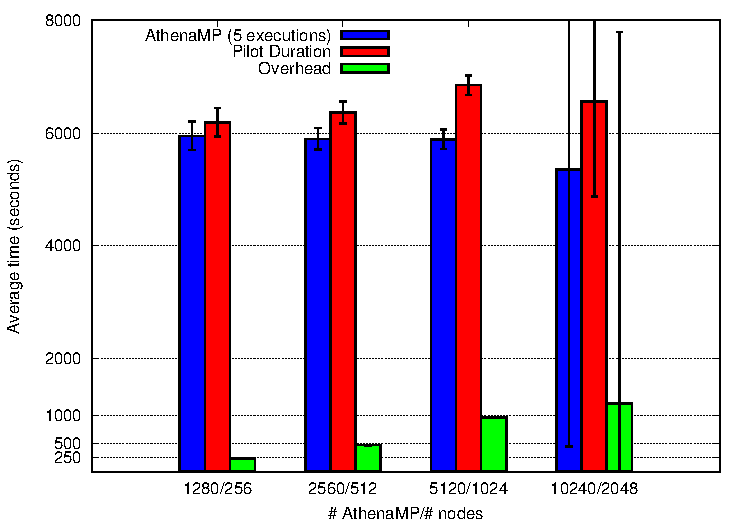
\includegraphics[height=4.5cm,width=\columnwidth]{./figures/NGE/weak2.pdf}
    \caption{Weak scalability with multiple generations: average pilot duration, average duration of five sequential AthenaMP executions and pilot's overhead for different pilot sizes (256, 512, 1024 and 2048 nodes). Note that the overhead refers to the axis on the right and it is expressed in tenths of a second.}
\label{fig:weakScal2a}
\end{figure}
%\begin{figure}[!htb]
%        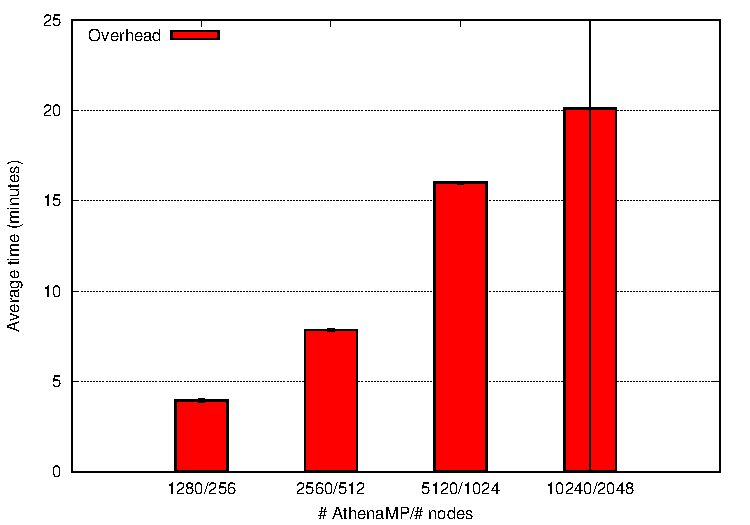
\includegraphics[width=0.4\textwidth]{./figures/NGE/weakOver2.pdf}
%    \caption{Weak scalability with multiple generations: average overhead by running AthenaMP on 256, 512, 1024 and 2048 nodes.}
%\label{fig:weakScal2b}
%\end{figure}
\subsubsection{Strong scalability}
The last experiments deals with strong scalability. Therefore, we run the same amount of tasks for different pilot sizes. 
We used a number of AthenaMP instances equal to 2048 and tested pilots with 256, 512, 1024 and 2048 nodes. Thus, the number of sequential AthenaMP instances is equal to eight for the smallest pilot and is null for the largest.  
Each AthenaMP instance simulates sixteen events as the previous experiment.

Figure \ref{fig:strongScala} depicts the average pilot duration and  the average execution time of possibly sequential AthenaMP instances.  We can notice that the difference between the pilot duration and the AthenaMP execution times is almost constant for all the pilot sizes although the overall duration of the pilot decreases linearly with the pilot size.

\begin{figure}[!htb]
        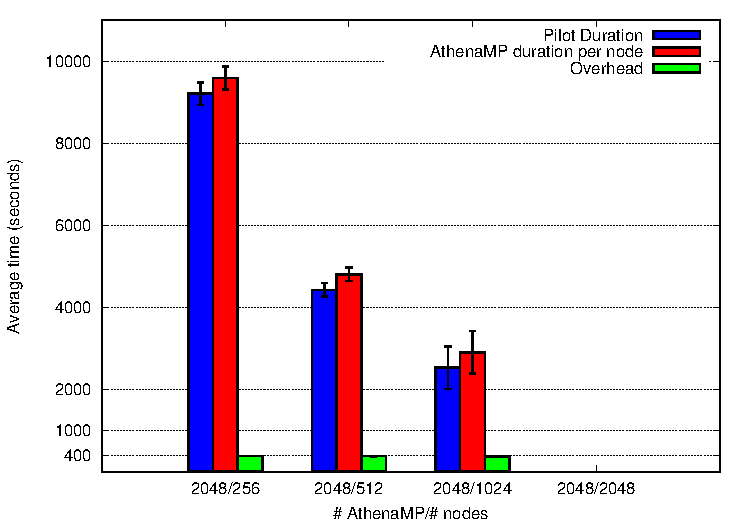
\includegraphics[height=4.5cm,width=\columnwidth]{./figures/NGE/strong.pdf}
    \caption{Strong scalability:  average pilot duration, average duration of sequential AthenaMP executions and pilot's overhead for different pilot sizes (256, 512, 1024 and 2048 nodes). Note that the overhead refers to the axis on the right and it is expressed in tenths of a second.}
\label{fig:strongScala}
\end{figure}



%
%\begin{figure}[!htb]
%        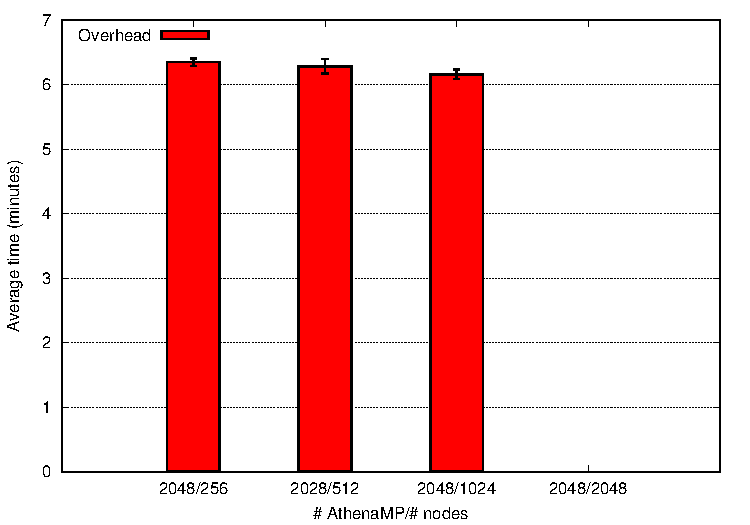
\includegraphics[width=0.4\textwidth]{./figures/NGE/strongOver.pdf}
%    \caption{Strong scalability: average overhead running AthenaMP on 256, 512, 1024 and 2048 nodes.}
%\label{fig:strongScalb}
%\end{figure}

 
%\subsubsection{Heterogeneous execution}
%
%The last experiment provides a proof of concept about the ability of the NGE to execute heterogeneous workload.
%In particular, we coupled the execution of AthenaMP with the execution of Gromacs to simulate molecular dynamics. 
%We performed the experiment by executing at first one AthenaMP per node and then, submitting a Gromacs simulation per core. Each Gromacs simulation requires ~20 minutes.
%We tested the following pilot sizes : 8, 16, 32, 64. 
%
%\begin{figure}[!htb]
%        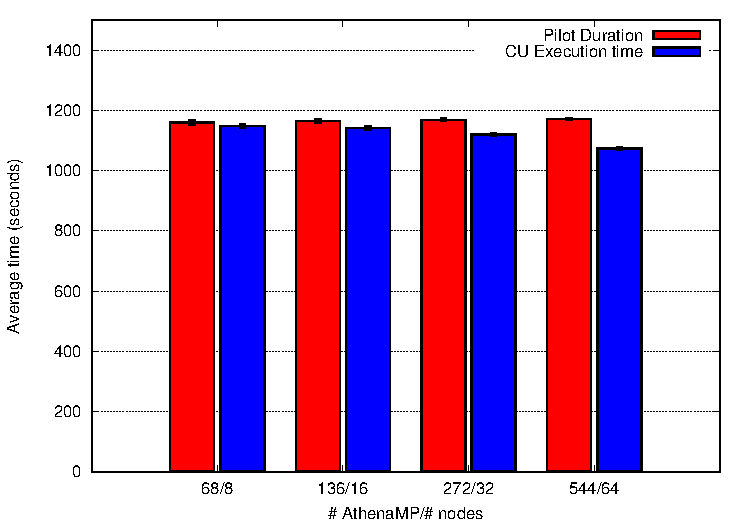
\includegraphics[width=0.5\textwidth]{./figures/NGE/MDET.pdf}
%    \caption{Average pilot execution time against average AthenaMP execution times  for pilot sizes: 256, 512, 1024 and 2048.}
%\label{fig:strongScala}
%\end{figure}
%\begin{figure}[!htb]
%        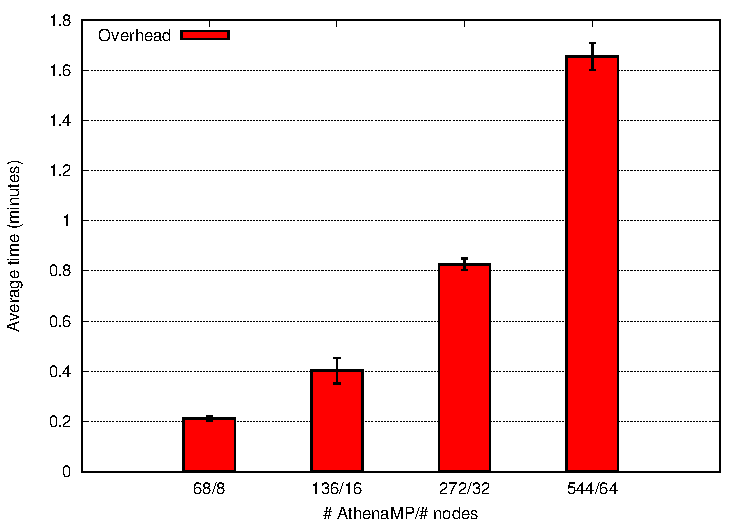
\includegraphics[width=0.5\textwidth]{./figures/NGE/MDOver.pdf}
%    \caption{Average overhead running AthenaMP for pilot sizes: 256, 512, 1024 and 2048.}
%\label{fig:MDScal}
%\end{figure}

% For this reason, the second set of the experiments aims to find
%sub-optimal parameters with which we can minimize the trade-off between the size
%of a slot and the time spent in queue waiting for that slot to become available.
%In other words, we aim to minimize the completion time by finding the best
%trade-off between execution time and queue time.
%
%This execution model introduces slot utilization as one of the key factors for
%high-performances. This happens because, in order to minimize the time spent in
%queue, we might asks for slots in advance and, then we could not be able to
%saturate them when they become available. Thus, this strategy requires a new
%functionality that allows the job to receive and execute new events while it is
%already running on the resources. In order to do that we perform the experiments
%by using a new generation executor that implements such functionality.
%
%As last observation, it is important to point out that the percentage of
%utilization of a slot is minor problem with the current implementation because,
%due to the dynamics of the Backfill queue, PanDA has a high probability to
%re-acquire a slot immediately after it has released one\aanote{Are we able to
%quantify this ``immediately''?}.
